\documentclass{beamer}
\usepackage[utf8]{inputenc}
\usepackage{amsmath, amssymb, bm}
\usepackage{physics}
\usepackage{graphicx}
\usepackage{hyperref}
\usepackage{tikz}
\usetheme{Madrid} % You can change the theme as you like
\usecolortheme{seagull}

\title[Quantum Computing and ML]{\textbf{Quantum Technology and Artificial Intelligence}}
\author{Morten Hjorth-Jensen}
\institute{Department of Physics and Center for Computing in Science Education, University of Oslo, Norway}
\date{Dscience seminar, UiO, April 3, 2025}

\begin{document}

%-----------------------------------------------------------
\begin{frame}
    \titlepage
\end{frame}

%-----------------------------------------------------------
\begin{frame}{Outline}
\tableofcontents
\end{frame}

%-----------------------------------------------------------
\section{Introduction to Quantum Computing}
\begin{frame}{What is Quantum Computing?}
Quantum computing leverages principles of quantum mechanics to perform computations beyond classical capabilities.

\vspace{10pt}
\textbf{Key Concepts:}
\begin{itemize}
    \item \textbf{Superposition:} Qubits can exist in a combination of states.
    \item \textbf{Entanglement:} Correlation between qubits regardless of distance.
    \item \textbf{Quantum Interference:} Probability amplitudes interfere to solve problems.
\end{itemize}

\pause
\textbf{Qubit Representation:}
\[
\ket{\psi} = \alpha \ket{0} + \beta \ket{1}, \quad |\alpha|^2 + |\beta|^2 = 1
\]
\end{frame}

%-----------------------------------------------------------
\section{Introduction to Machine Learning}
\begin{frame}{What is Machine Learning?}
Machine Learning (ML) is the study of algorithms that improve through data experience.

\textbf{Types of Machine Learning:}
\begin{itemize}
    \item \textbf{Supervised Learning:} Labeled data for classification or regression.
    \item \textbf{Unsupervised Learning:} No labels; discover hidden patterns.
    \item \textbf{Reinforcement Learning:} Learning through interaction with the environment.
\end{itemize}

\pause
\textbf{ML Workflow:}
\[
\text{Data} \rightarrow \text{Model Training} \rightarrow \text{Prediction}
\]
\end{frame}

%-----------------------------------------------------------
\section{Quantum Machine Learning (QML)}
\begin{frame}{What is Quantum Machine Learning?}
\textbf{Quantum Machine Learning (QML)} integrates quantum computing with machine learning algorithms to exploit quantum advantages.

\vspace{10pt}
\textbf{Motivation:}
\begin{itemize}
    \item High-dimensional Hilbert spaces for better feature representation.
    \item Quantum parallelism for faster computation.
    \item Quantum entanglement for richer data encoding.
\end{itemize}

\pause
\textbf{Quantum Model Example:}
\[
U(\theta)\ket{x} \implies \text{Quantum Kernel for Classification}
\]
\end{frame}





\begin{frame}[plain,fragile]
\frametitle{AI/ML and some statements you may have heard (and what do they mean?)}

https://www.businessenergyuk.com/knowledge-hub/chatgpt-energy-consumption-visualized/



\begin{enumerate}
\item Fei-Fei Li on ImageNet: \textbf{map out the entire world of objects} (\href{{https://cacm.acm.org/news/219702-the-data-that-transformed-ai-research-and-possibly-the-world/fulltext}}{The data that transformed AI research})

\item Russell and Norvig in their popular textbook: \textbf{relevant to any intellectual task; it is truly a universal field} (\href{{http://aima.cs.berkeley.edu/}}{Artificial Intelligence, A modern approach})

\item Woody Bledsoe puts it more bluntly: \textbf{in the long run, AI is the only science} (quoted in Pamilla McCorduck, \href{{https://www.pamelamccorduck.com/machines-who-think}}{Machines who think})
\end{enumerate}

\noindent
If you wish to have a critical read on AI/ML from a societal point of view, see \href{{https://www.katecrawford.net/}}{Kate Crawford's recent text Atlas of AI}.

\textbf{Here: with AI/ML we intend a collection of machine learning methods with an emphasis on statistical learning and data analysis}
\end{frame}

\begin{frame}[plain,fragile]
\frametitle{Curse of dimensionality}

\vspace{6mm}

% inline figure
\centerline{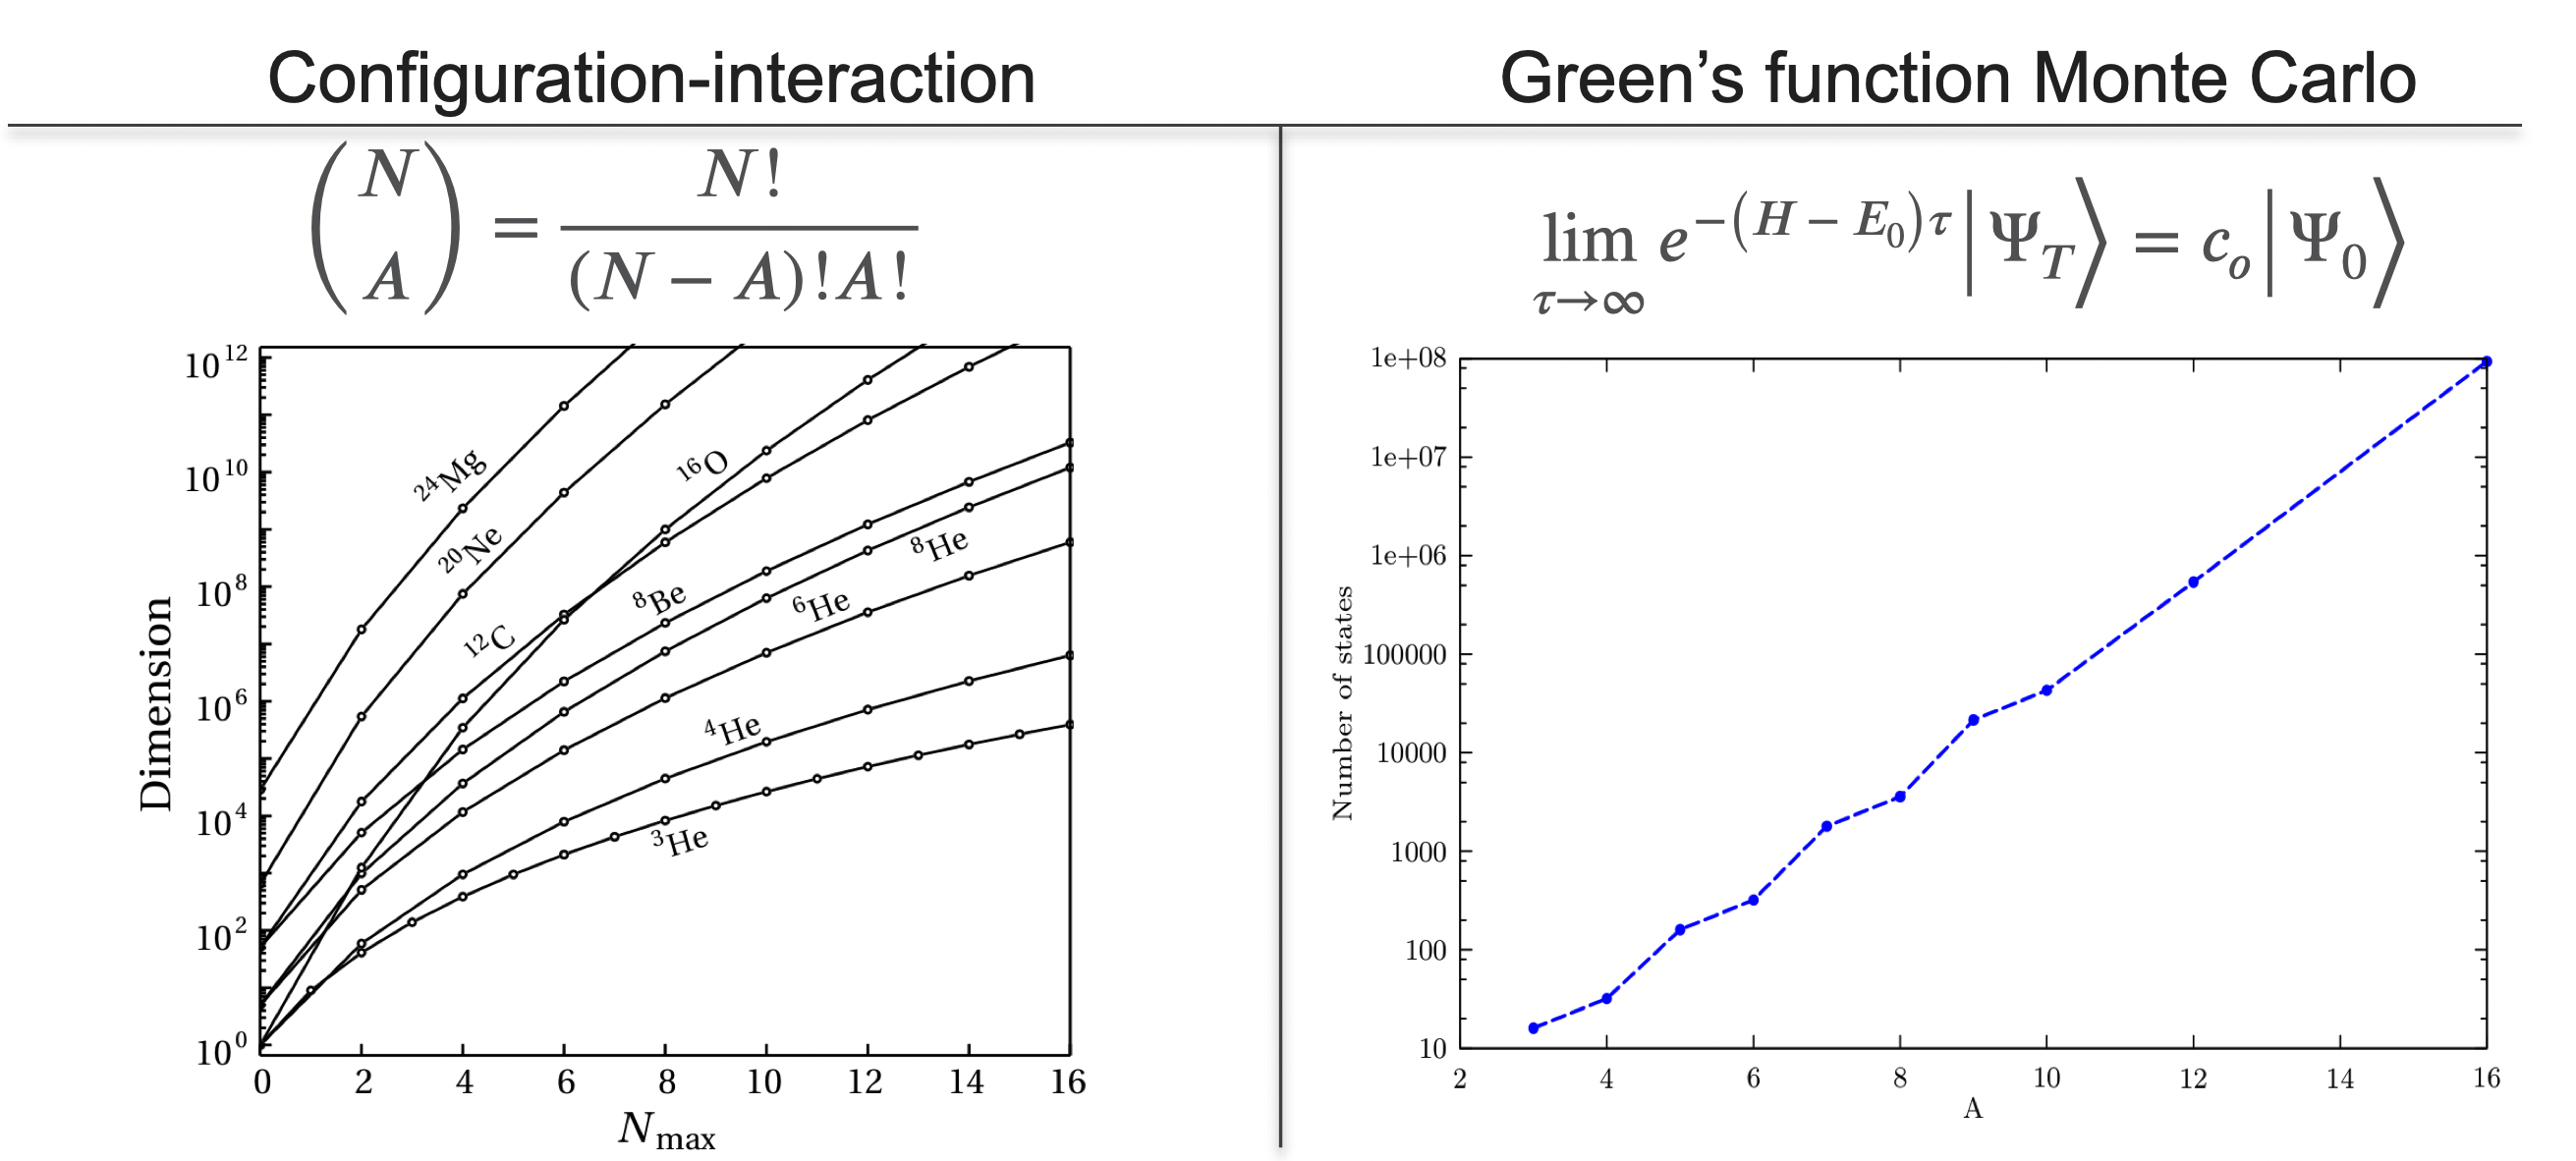
\includegraphics[width=1.0\linewidth]{figures/mbpfig2.png}}

\vspace{6mm}
\end{frame}

\begin{frame}[plain,fragile]
\frametitle{Neural network quantum states}

\begin{block}{Neural networks compactly represent complex high-dimensional functions }
Most quantum states of interest have distinctive features and intrinsic structures
%FIGURE: [figures/mbpfig3.png, width=900 frac=1.0]
\end{block}
\end{frame}

\begin{frame}[plain,fragile]
\frametitle{Machine learning. A simple perspective on the interface between ML and Physics}

\vspace{6mm}

% inline figure
\centerline{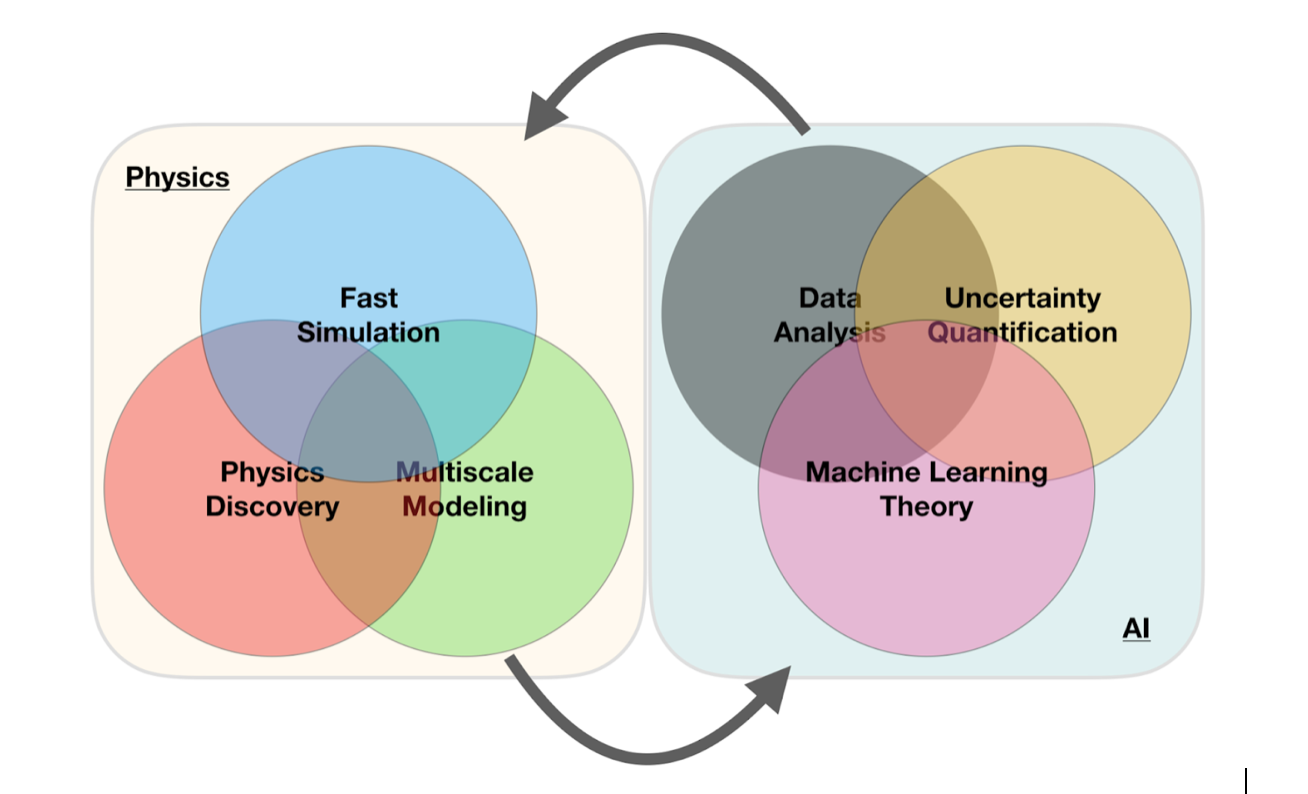
\includegraphics[width=1.0\linewidth]{figures/mlimage.png}}

\vspace{6mm}
\end{frame}

\begin{frame}[plain,fragile]
\frametitle{Types of machine learning}

\begin{block}{}
The approaches to machine learning are many, but are often split into two main categories. 
In \emph{supervised learning} we know the answer to a problem,
and let the computer deduce the logic behind it. On the other hand, \emph{unsupervised learning}
is a method for finding patterns and relationship in data sets without any prior knowledge of the system.

An important  third category is  \emph{reinforcement learning}. This is a paradigm 
of learning inspired by behavioural psychology, where learning is achieved by trial-and-error, 
solely from rewards and punishment.
\end{block}
\end{frame}

\begin{frame}[plain,fragile]
\frametitle{Main categories}

\begin{block}{}
Another way to categorize machine learning tasks is to consider the desired output of a system.
Some of the most common tasks are:

\begin{itemize}
  \item Classification: Outputs are divided into two or more classes. The goal is to   produce a model that assigns inputs into one of these classes. An example is to identify  digits based on pictures of hand-written ones. Classification is typically supervised learning.

  \item Regression: Finding a functional relationship between an input data set and a reference data set.   The goal is to construct a function that maps input data to continuous output values.

  \item Clustering: Data are divided into groups with certain common traits, without knowing the different groups beforehand.  It is thus a form of unsupervised learning.
\end{itemize}

\noindent
\end{block}
\end{frame}

\begin{frame}[plain,fragile]
\frametitle{The plethora  of machine learning algorithms/methods}

\begin{enumerate}
\item Deep learning: Neural Networks (NN), Convolutional NN, Recurrent NN, Boltzmann machines, autoencoders and variational autoencoders  and generative adversarial networks, stable diffusion and many more generative models

\item Bayesian statistics and Bayesian Machine Learning, Bayesian experimental design, Bayesian Regression models, Bayesian neural networks, Gaussian processes and much more

\item Dimensionality reduction (Principal component analysis), Clustering Methods and more

\item Ensemble Methods, Random forests, bagging and voting methods, gradient boosting approaches 

\item Linear and logistic regression, Kernel methods, support vector machines and more

\item Reinforcement Learning; Transfer Learning and more 
\end{enumerate}

\noindent
\end{frame}

\begin{frame}[plain,fragile]
\frametitle{Example of discriminative modeling, \href{{https://www.oreilly.com/library/view/generative-deep-learning/9781098134174/ch01.html}}{taken from Generative Deep Learning by David Foster}}

\vspace{6mm}

% inline figure
\centerline{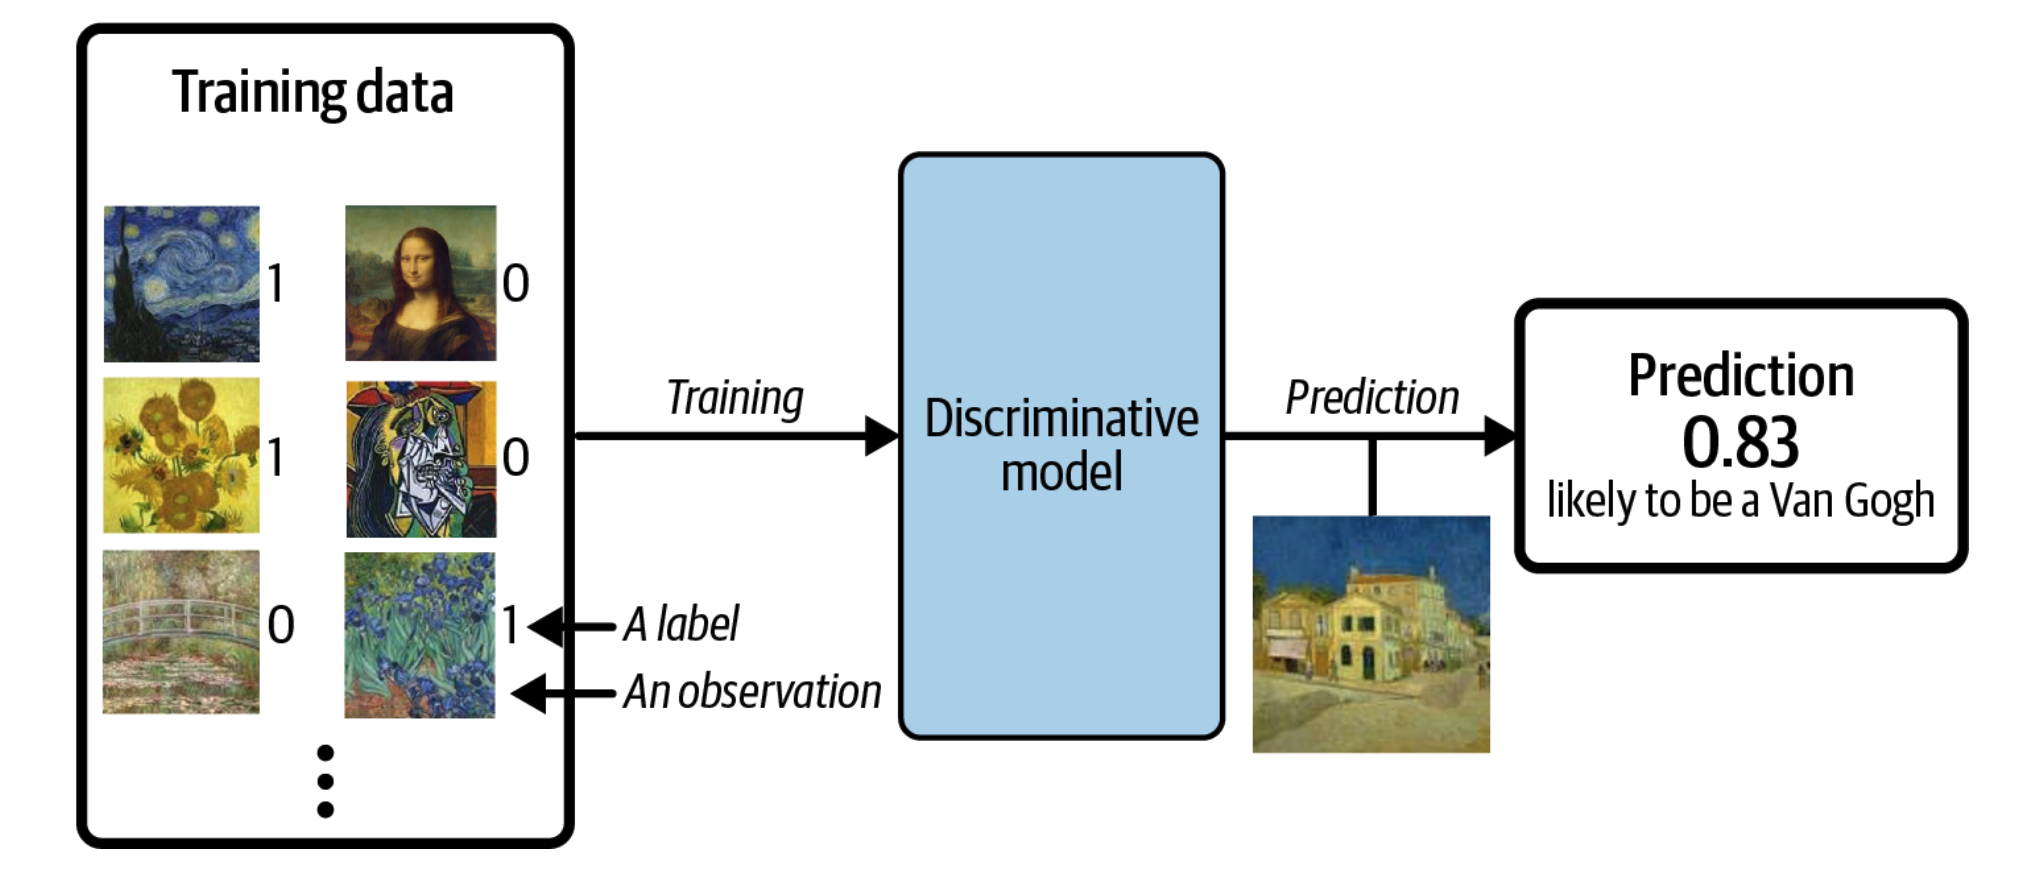
\includegraphics[width=1.0\linewidth]{figures/standarddeeplearning.png}}

\vspace{6mm}
\end{frame}

\begin{frame}[plain,fragile]
\frametitle{Example of generative modeling, \href{{https://www.oreilly.com/library/view/generative-deep-learning/9781098134174/ch01.html}}{taken from Generative Deep Learning by David Foster}}

\vspace{6mm}

% inline figure
\centerline{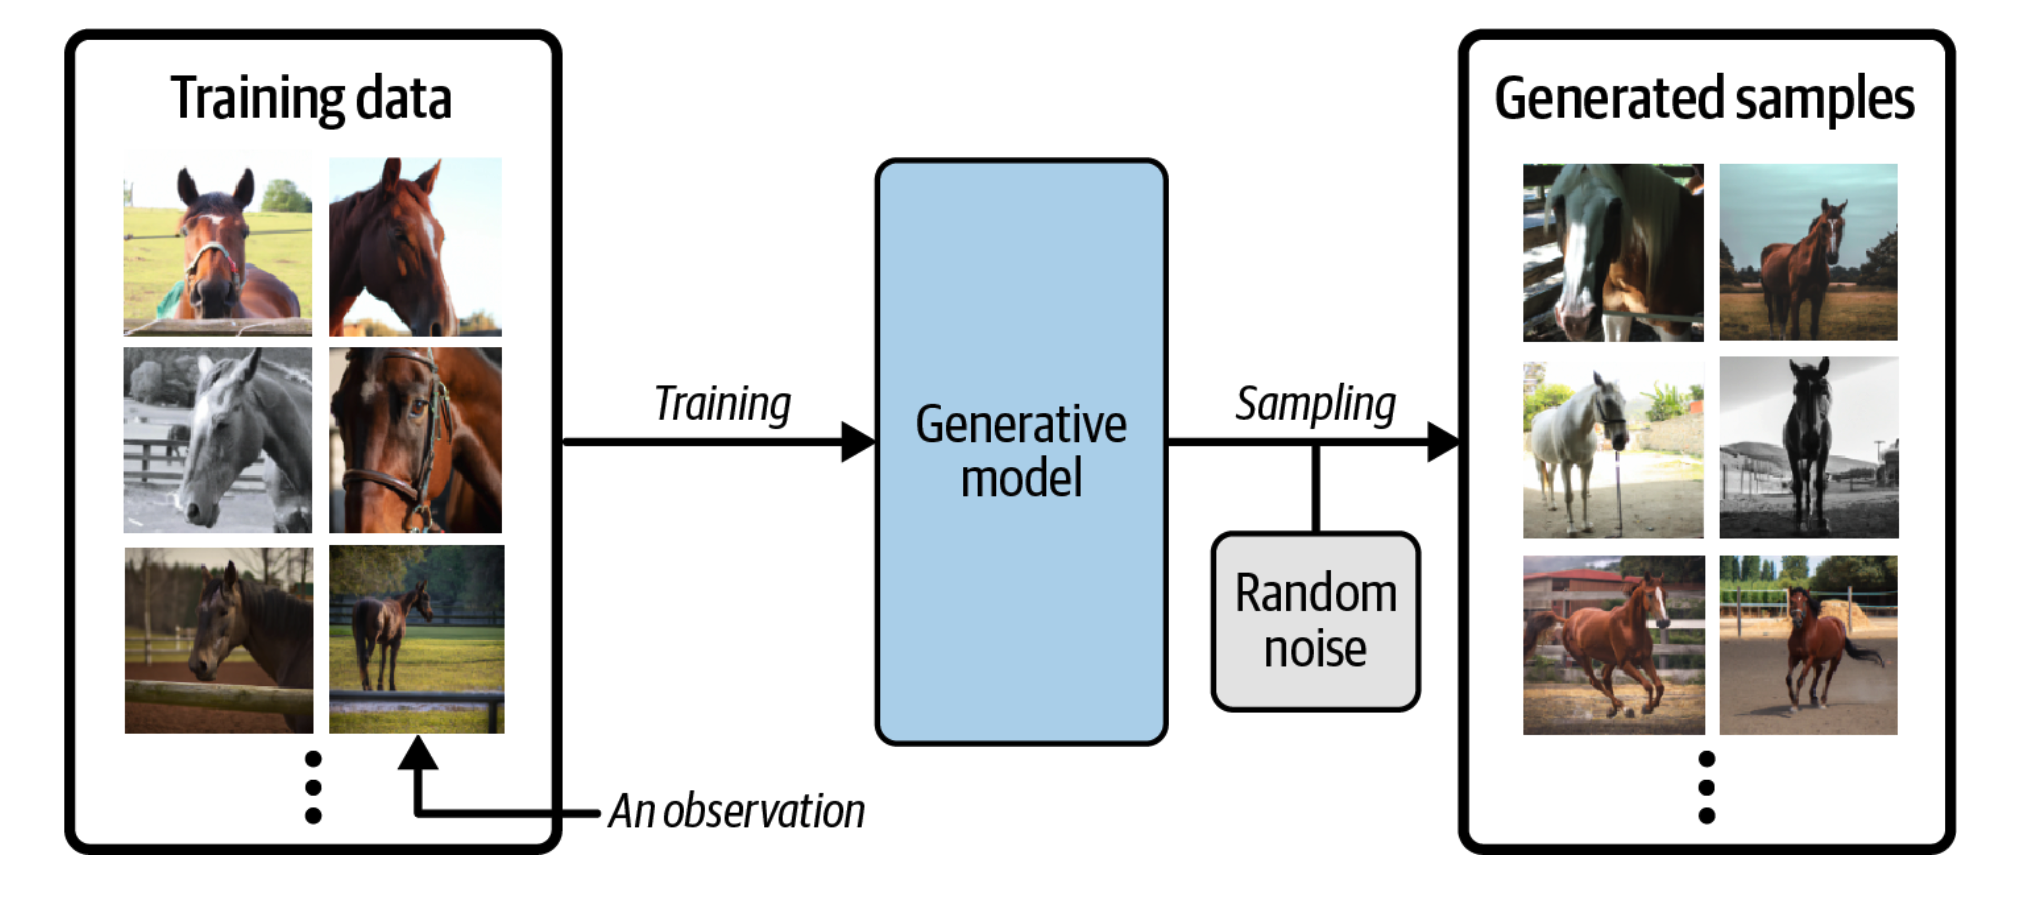
\includegraphics[width=1.0\linewidth]{figures/generativelearning.png}}

\vspace{6mm}
\end{frame}

\begin{frame}[plain,fragile]
\frametitle{Taxonomy of generative deep learning, \href{{https://www.oreilly.com/library/view/generative-deep-learning/9781098134174/ch01.html}}{taken from Generative Deep Learning by David Foster}}

\vspace{6mm}

% inline figure
\centerline{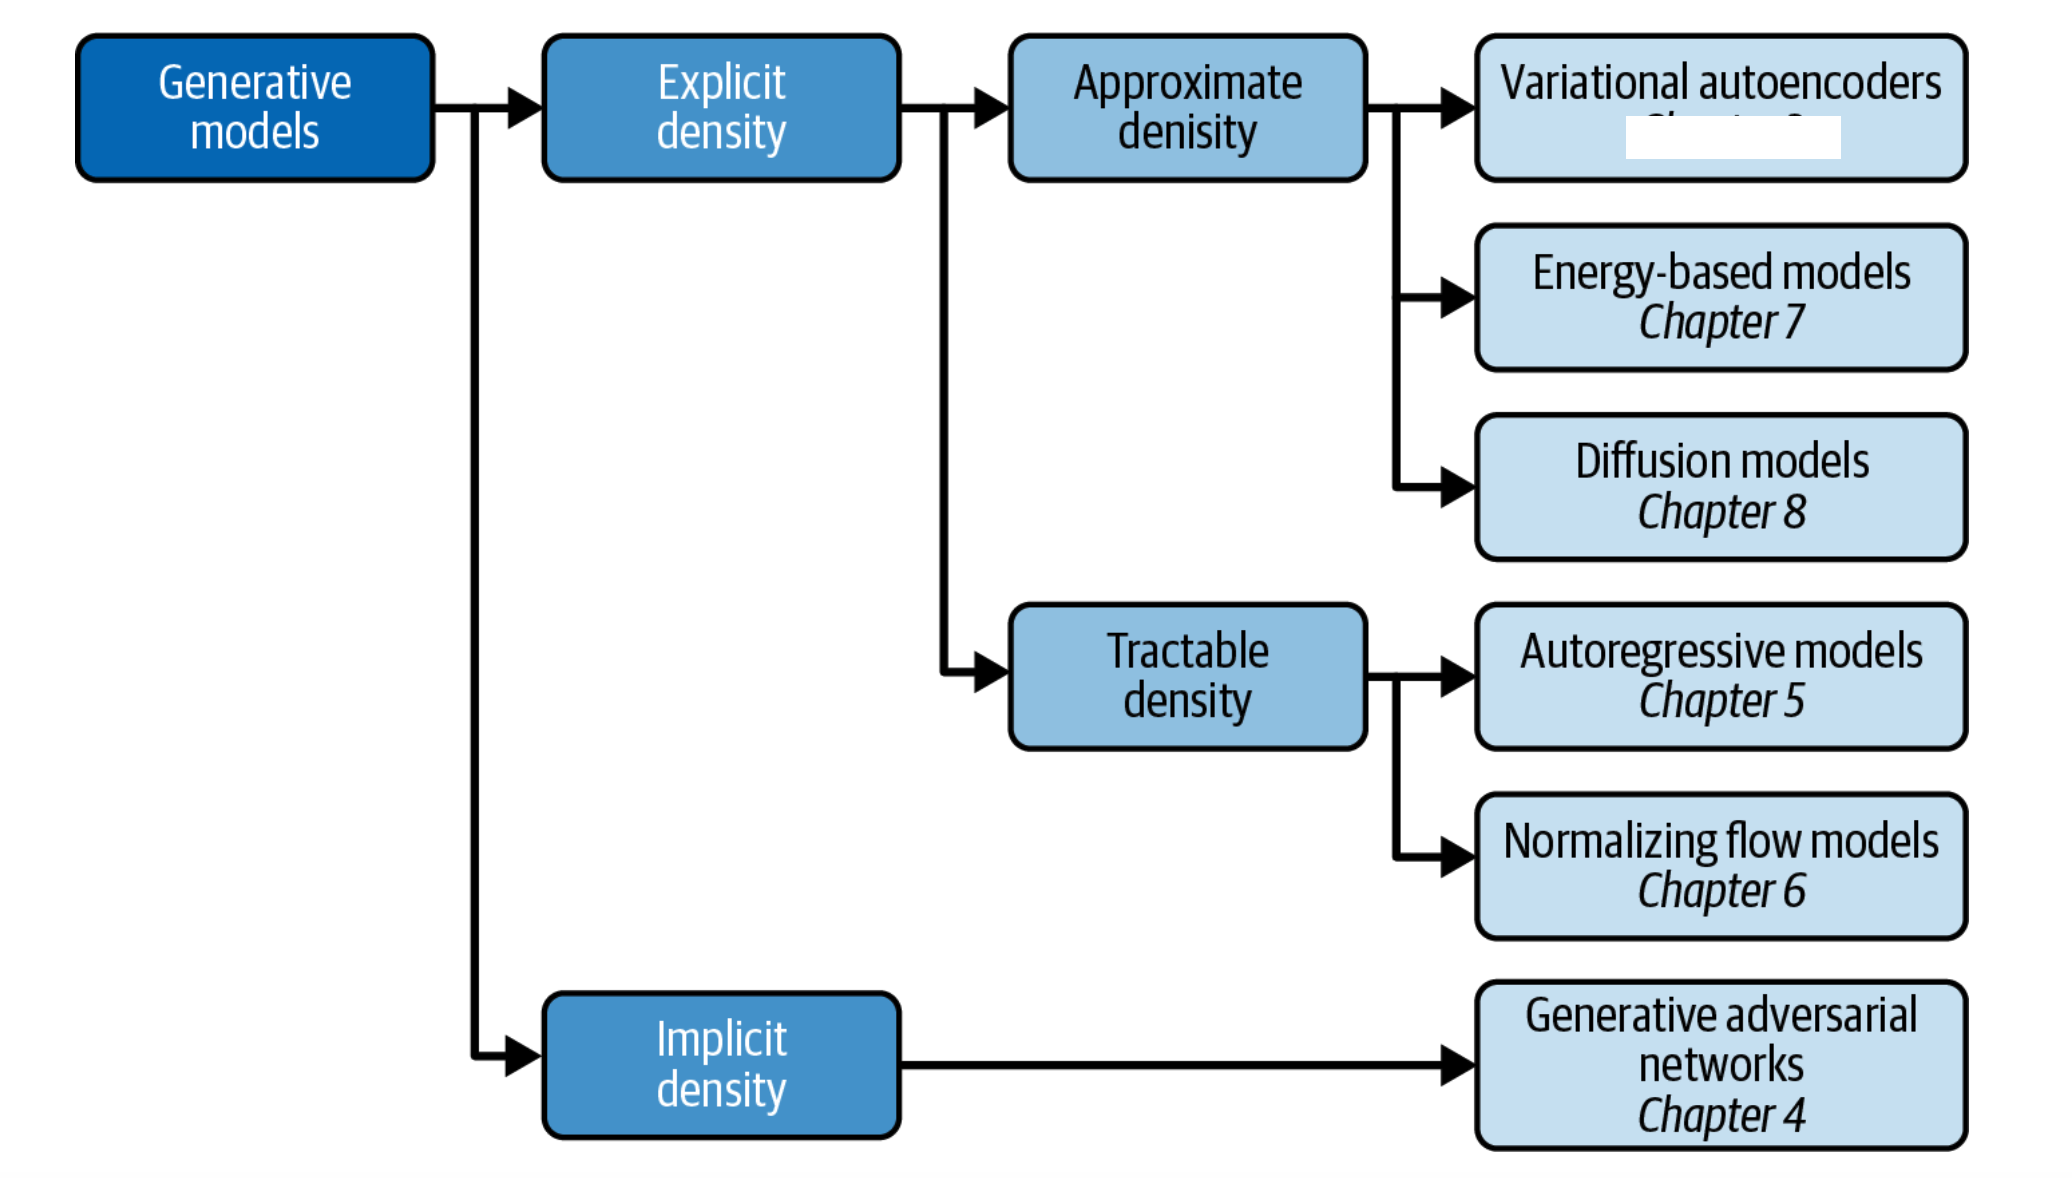
\includegraphics[width=1.0\linewidth]{figures/generativemodels.png}}

\vspace{6mm}
\end{frame}


\begin{frame}[plain,fragile]
\frametitle{What are the basic Machine Learning ingredients?}

\begin{block}{}
Almost every problem in ML and data science starts with the same ingredients:
\begin{itemize}
\item The dataset $\bm{x}$ (could be some observable quantity of the system we are studying)

\item A model which is a function of a set of parameters $\bm{\alpha}$ that relates to the dataset, say a likelihood  function $p(\bm{x}\vert \bm{\alpha})$ or just a simple model $f(\bm{\alpha})$

\item A so-called \textbf{loss/cost/risk} function $\mathcal{C} (\bm{x}, f(\bm{\alpha}))$ which allows us to decide how well our model represents the dataset. 
\end{itemize}

\noindent
We seek to minimize the function $\mathcal{C} (\bm{x}, f(\bm{\alpha}))$ by finding the parameter values which minimize $\mathcal{C}$. This leads to  various minimization algorithms. It may surprise many, but at the heart of all machine learning algortihms there is an optimization problem. 
\end{block}
\end{frame}

\begin{frame}[plain,fragile]
\frametitle{Low-level machine learning, the family of ordinary least squares methods}

Our data which we want to apply a machine learning method on, consist
of a set of inputs $\bm{x}^T=[x_0,x_1,x_2,\dots,x_{n-1}]$ and the
outputs we want to model $\bm{y}^T=[y_0,y_1,y_2,\dots,y_{n-1}]$.
We assume  that the output data can be represented (for a regression case) by a continuous function $f$
through
\[
\bm{y}=f(\bm{x})+\bm{\epsilon}.
\]
\end{frame}

\begin{frame}[plain,fragile]
\frametitle{Setting up the equations}

In linear regression we approximate the unknown function with another
continuous function $\tilde{\bm{y}}(\bm{x})$ which depends linearly on
some unknown parameters
$\bm{\theta}^T=[\theta_0,\theta_1,\theta_2,\dots,\theta_{p-1}]$.

The input data can be organized in terms of a so-called design matrix 
with an approximating function $\bm{\tilde{y}}$ 
\[
\bm{\tilde{y}}= \bm{X}\bm{\theta},
\]
\end{frame}

\begin{frame}[plain,fragile]
\frametitle{The objective/cost/loss function}

The  simplest approach is the mean squared error
\[
C(\bm{\Theta})=\frac{1}{n}\sum_{i=0}^{n-1}\left(y_i-\tilde{y}_i\right)^2=\frac{1}{n}\left\{\left(\bm{y}-\bm{\tilde{y}}\right)^T\left(\bm{y}-\bm{\tilde{y}}\right)\right\},
\]
or using the matrix $\bm{X}$ and in a more compact matrix-vector notation as
\[
C(\bm{\Theta})=\frac{1}{n}\left\{\left(\bm{y}-\bm{X}\bm{\theta}\right)^T\left(\bm{y}-\bm{X}\bm{\theta}\right)\right\}.
\]
This function represents one of many possible ways to define the so-called cost function.
\end{frame}

\begin{frame}[plain,fragile]
\frametitle{Training solution}

Optimizing with respect to the unknown parameters $\theta_j$ we get 
\[
\bm{X}^T\bm{y} = \bm{X}^T\bm{X}\bm{\theta},  
\]
and if the matrix $\bm{X}^T\bm{X}$ is invertible we have the optimal values
\[
\hat{\bm{\theta}} =\left(\bm{X}^T\bm{X}\right)^{-1}\bm{X}^T\bm{y}.
\]

We say we 'learn' the unknown parameters $\bm{\theta}$ from the last equation.
\end{frame}















%-----------------------------------------------------------
\section{Quantum Algorithms for ML}
\begin{frame}{1. Quantum Support Vector Machines (QSVM)}
\textbf{Quantum Kernel Estimation:}
\begin{itemize}
    \item Maps classical data to a quantum Hilbert space.
    \item Quantum kernel measures similarity in high-dimensional space.
\end{itemize}

\pause
\textbf{Quantum Kernel:}
\[
K(x, x') = |\braket{\psi(x) | \psi(x')}|^2
\]

\textbf{Advantage:}
- Potentially exponential speedup over classical SVMs.
\end{frame}

%-----------------------------------------------------------
\begin{frame}{2. Quantum Neural Networks (QNNs)}
\textbf{Quantum Neural Networks} replace classical neurons with parameterized quantum circuits.

\textbf{Key Concepts:}
\begin{itemize}
    \item Quantum Gates as Activation Functions.
    \item Variational Quantum Circuits (VQCs) for optimization.
\end{itemize}

\pause
\textbf{Parameterized Quantum Circuit:}
\[
U(\theta) = \prod_i R_y(\theta_i) \cdot CNOT \cdot R_x(\theta_i)
\]

\textbf{Advantage:}
- Quantum gradients enable exploration of non-convex landscapes.
\end{frame}

%-----------------------------------------------------------
\begin{frame}{3. Quantum Boltzmann Machines (QBMs)}
\textbf{Quantum Boltzmann Machines} leverage quantum mechanics to sample from a probability distribution.

\begin{itemize}
    \item Quantum tunneling aids in escaping local minima.
    \item Quantum annealing for optimization problems.
\end{itemize}

\pause
\textbf{Quantum Hamiltonian:}
\[
H = -\sum_i b_i \sigma_i^z - \sum_{ij} w_{ij} \sigma_i^z \sigma_j^z
\]

\textbf{Advantage:}
- Efficient sampling in complex probability distributions.
\end{frame}

%-----------------------------------------------------------
\section{Quantum Speedups}
\begin{frame}{Quantum Speedups in ML}
\textbf{Why Quantum?}
\begin{itemize}
    \item \textbf{Quantum Parallelism:} Process multiple states simultaneously.
    \item \textbf{Quantum Entanglement:} Correlated states for richer information.
    \item \textbf{Quantum Interference:} Constructive and destructive interference to enhance solutions.
\end{itemize}

\pause
\textbf{Example - Grover's Algorithm:}
\[
\text{Quantum Search Complexity: } O(\sqrt{N}) \text{ vs. } O(N)
\]

\textbf{Advantage:}
- Speedups in high-dimensional optimization and linear algebra problems.
\end{frame}

%-----------------------------------------------------------
\section{Challenges in Quantum Machine Learning}
\begin{frame}{Challenges and Limitations}
\textbf{1. Quantum Hardware Limitations:}
\begin{itemize}
    \item Noisy Intermediate-Scale Quantum (NISQ) devices.
    \item Decoherence and limited qubit coherence times.
\end{itemize}

\textbf{2. Data Encoding:}
\begin{itemize}
    \item Efficient embedding of classical data into quantum states.
\end{itemize}

\textbf{3. Scalability:}
\begin{itemize}
    \item Difficult to scale circuits to large datasets.
\end{itemize}
\end{frame}

%-----------------------------------------------------------
\section{Applications of QML}
\begin{frame}{Applications of Quantum Machine Learning}
\textbf{1. Quantum Chemistry:}
\begin{itemize}
    \item Simulate molecular structures with QML.
\end{itemize}

\textbf{2. Finance:}
\begin{itemize}
    \item Quantum optimization for portfolio management.
\end{itemize}

\textbf{3. Image Recognition:}
\begin{itemize}
    \item Quantum-enhanced convolutional neural networks.
\end{itemize}
\end{frame}

%-----------------------------------------------------------
\section{Future Perspectives}
\begin{frame}{Future Perspectives in QML}
\textbf{1. Fault-Tolerant Quantum Computing:}
\begin{itemize}
    \item Overcoming noise for stable quantum circuits.
\end{itemize}

\textbf{2. Hybrid Quantum-Classical Models:}
\begin{itemize}
    \item Combining quantum circuits with classical neural networks.
\end{itemize}

\textbf{3. Quantum Internet:}
\begin{itemize}
    \item Distributed quantum machine learning over quantum networks.
\end{itemize}
\end{frame}


\end{document}




\begin{frame}[plain,fragile]
\frametitle{Scientific Machine Learning}

An important and emerging field is what has been dubbed as scientific ML, see the article by Deiana et al, Applications and Techniques for Fast Machine Learning in Science, Big Data \textbf{5}, 787421 (2022) \href{{https://doi.org/10.3389/fdata.2022.787421}}{\nolinkurl{https://doi.org/10.3389/fdata.2022.787421}}

\begin{block}{}
The authors discuss applications and techniques for fast machine
learning (ML) in science -- the concept of integrating power ML
methods into the real-time experimental data processing loop to
accelerate scientific discovery. The report covers three main areas

\begin{enumerate}
\item applications for fast ML across a number of scientific domains;

\item techniques for training and implementing performant and resource-efficient ML algorithms;

\item and computing architectures, platforms, and technologies for deploying these algorithms.
\end{enumerate}

\noindent
\end{block}
\end{frame}

\begin{frame}[plain,fragile]
\frametitle{ML for detectors}

\vspace{6mm}

% inline figure
\centerline{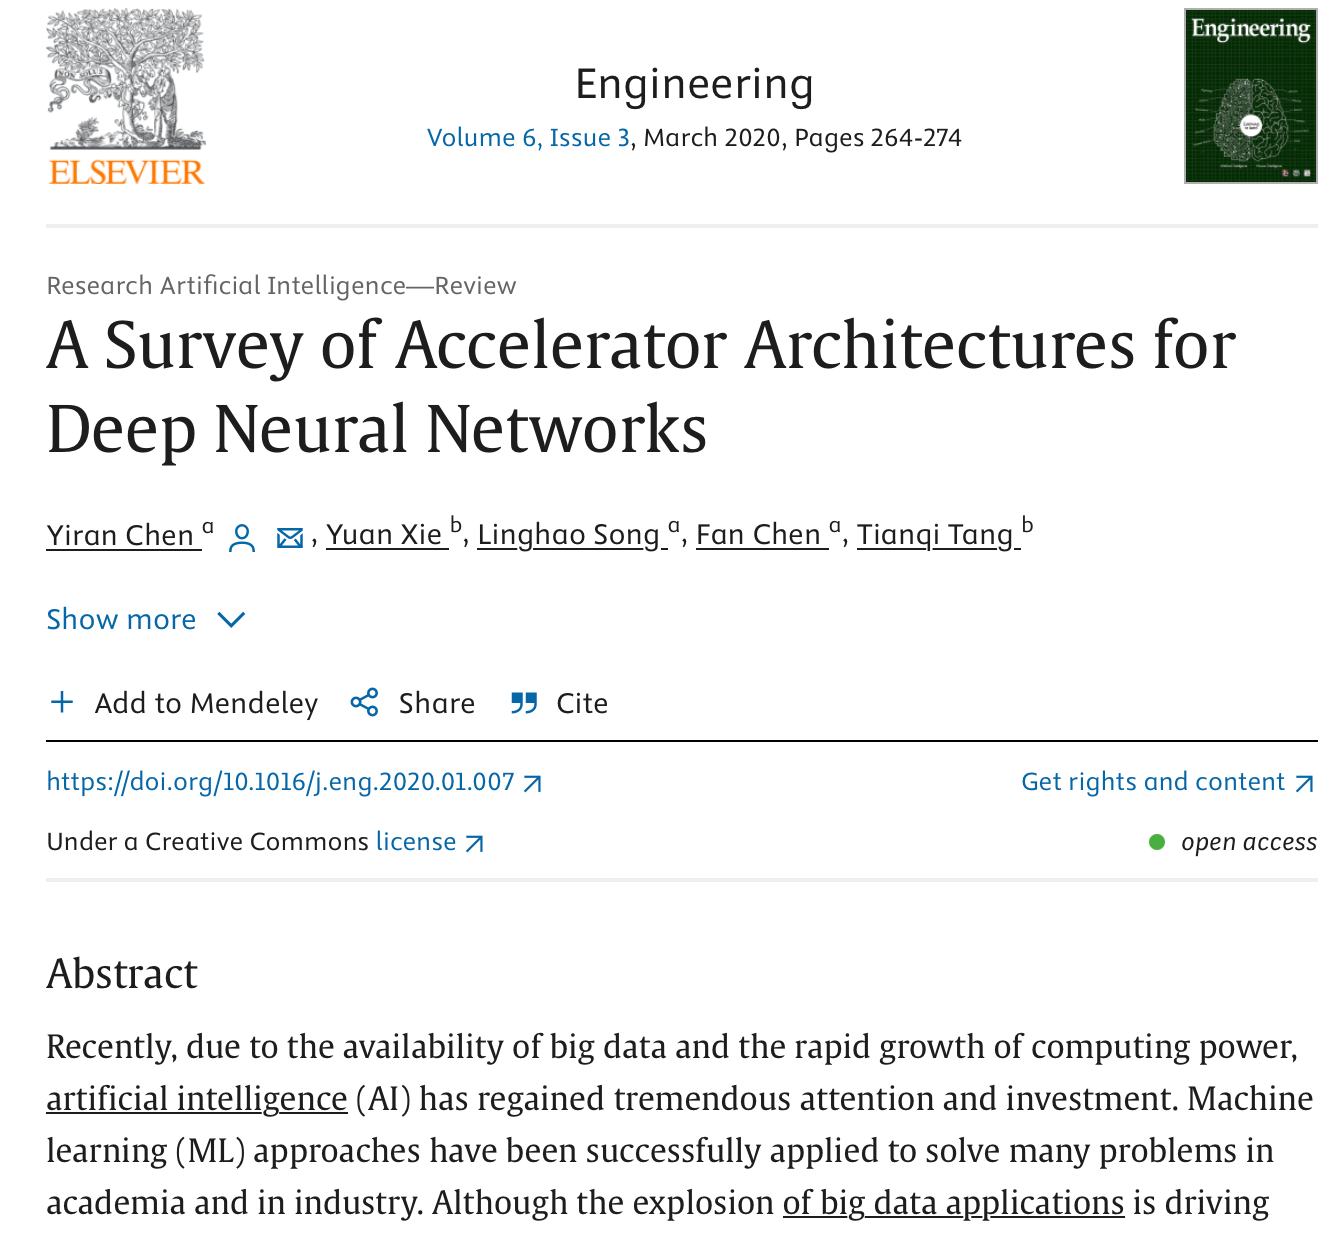
\includegraphics[width=1.0\linewidth]{figures/detectors.png}}

\vspace{6mm}
\end{frame}



\begin{frame}[plain,fragile]
\frametitle{Neutron star structure}

\vspace{6mm}

% inline figure
\centerline{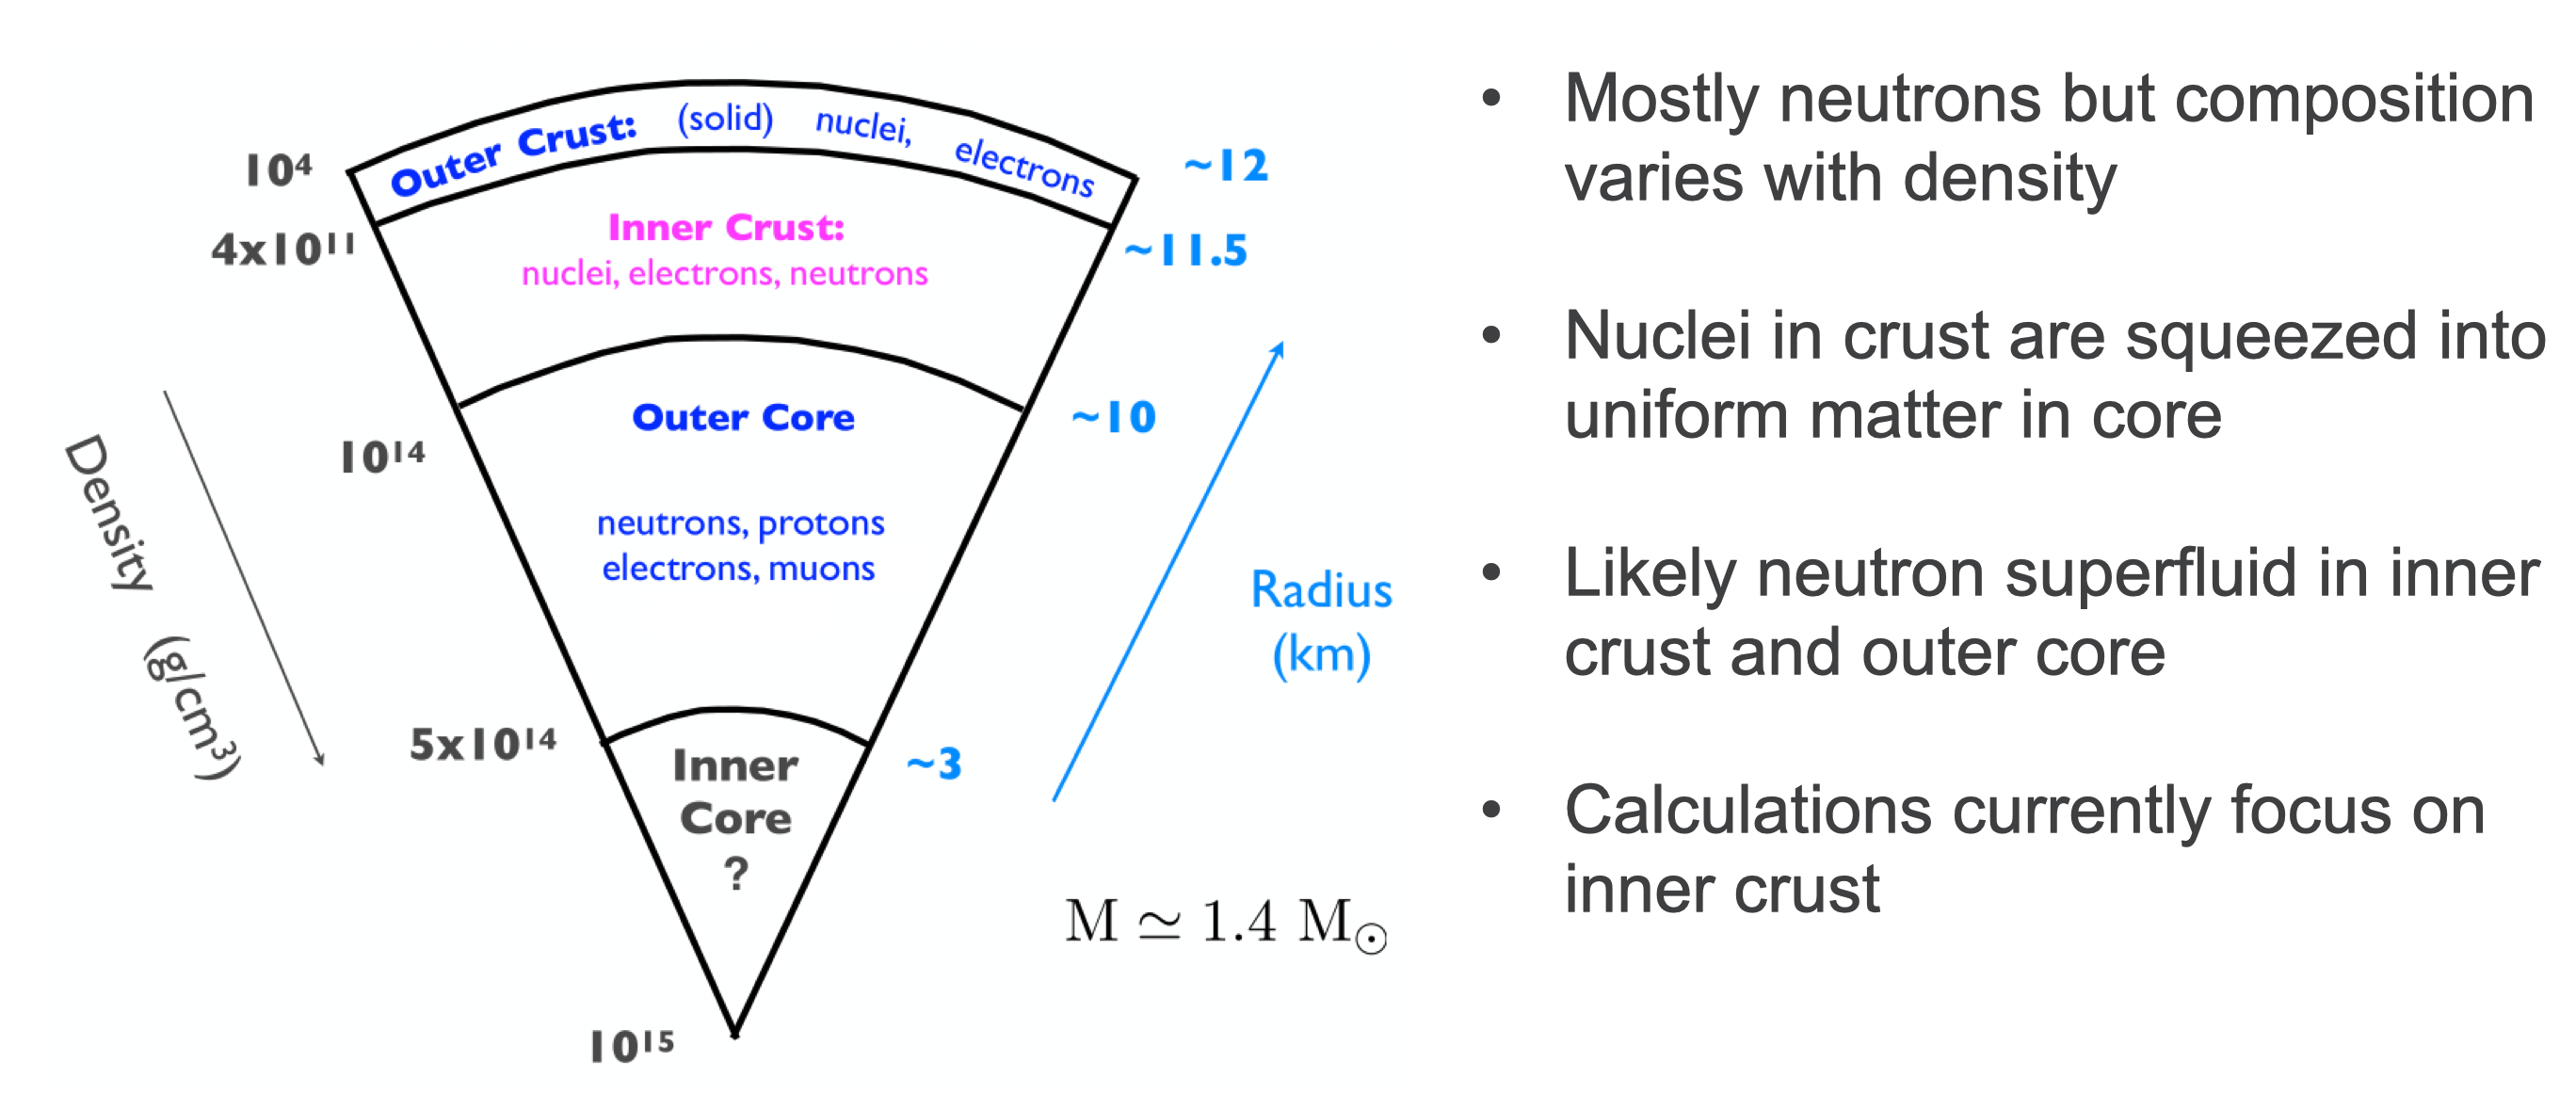
\includegraphics[width=1.0\linewidth]{figures/mbpfig5.png}}

\vspace{6mm}
\end{frame}

\begin{frame}[plain,fragile]
\frametitle{\href{{https://journals.aps.org/prresearch/pdf/10.1103/PhysRevResearch.5.033062}}{Dilute neutron star matter from neural-network quantum states by Fore et al, Physical Review Research 5, 033062 (2023)} at density $\rho=0.04$ fm$^{-3}$}

\begin{block}{}

\vspace{6mm}

% inline figure
\centerline{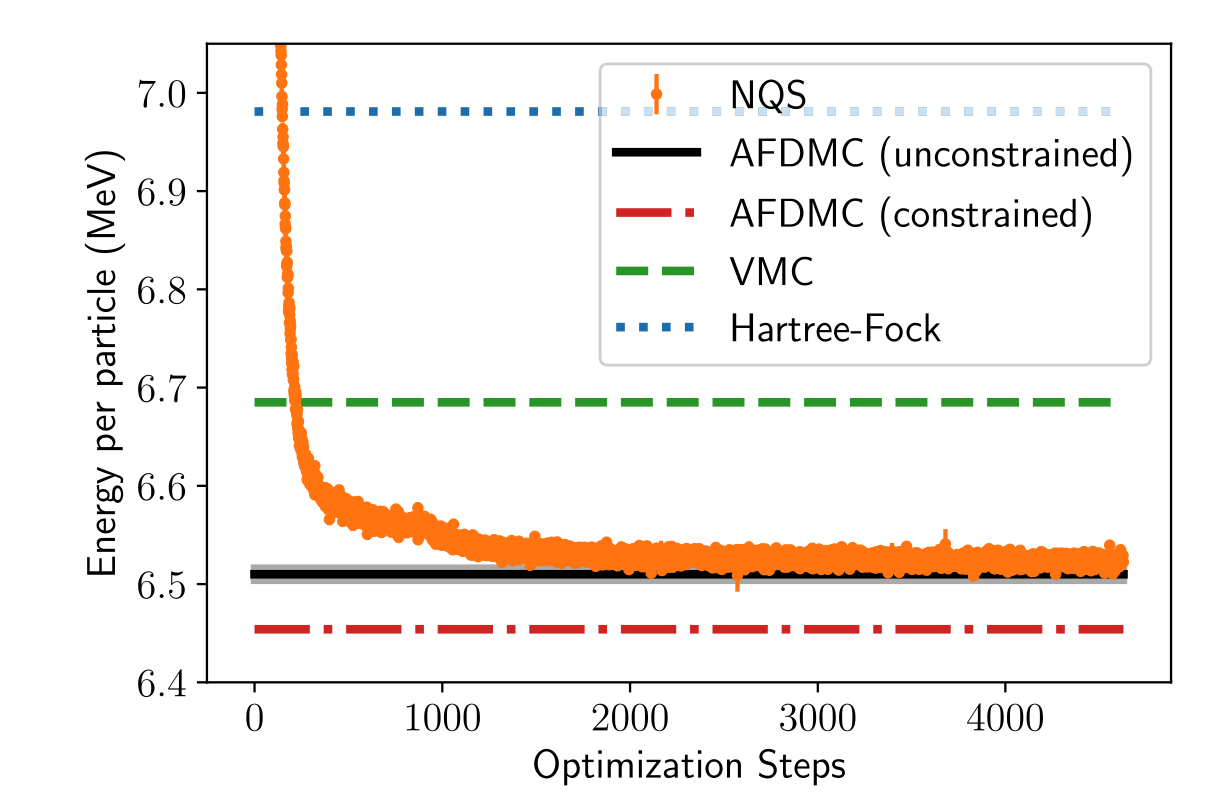
\includegraphics[width=0.9\linewidth]{figures/nmatter.png}}

\vspace{6mm}

\end{block}
\end{frame}

